\documentclass[10pt]{beamer}

\usecolortheme{dove}
\definecolor{mycyan}{rgb}{0.2157, 0.7059, 0.9608}
\setbeamercolor{alerted text}{fg=mycyan}
\setbeamertemplate{bibliography item}{\insertbiblabel}
\setbeamertemplate{caption}[numbered]
\hypersetup{colorlinks,linkcolor=,urlcolor=mycyan}
\usepackage{animate,xcolor,colortbl,nicefrac}
\usepackage[italian]{babel}
\usepackage{listings}
\lstset{upquote=false}
\usepackage[]{framed}
\begin{document}


\begin{frame}
  \title{Metodi di Krylov}
  \subtitle{Metodi per la soluzione numerica di sistemi di equazioni lineari applicabili in un sottospazio di Krylov.}
  \date{06/05/2020}
  \author[Principal]{Fabio Camagni \and Andrea Favero \and  \\Lorenzo Fiamingo \and Stefano Gallivanone \and Nazariy Nashkolnyy}
  \maketitle
\end{frame}

\begin{frame}
    \frametitle{Bibliografia}
    
  \begin{thebibliography}{99}\small
    \bibitem{quarteroni2012calcolo}
    Quarteroni, Saleri, and Gervasio.
    \newblock {\em Calcolo Scientifico: Esercizi e problemi risolti con MATLAB e  Octave}.
    \newblock UNITEXT. Springer Milan, 2012.

    \bibitem{trefethen-bau}
    Trefethen, and Bau.
    \newblock {\em Numerical Linear Algebra}.
    \newblock SIAM, 1997.
    
    \bibitem{dac95}
    Telichevesky, Kundert, and White.
    \newblock {\em Efficient Steady-State Analysis based on Matrix-Free Krylov-Subspace Methods}.
    \newblock {\em Scientific report}, June 1995.

   \end{thebibliography}

%Una volta inserito un documento in bibliografia, 
%può essere citato così:~\cite{quarteroni2012calcolo}
  
\end{frame}  

\begin{frame}
  \frametitle{Sommario}
  %Questo comando inserisce una lista delle sezioni in
  %cui è divisa la presentazione. Perché una sezione appaia 
  %nel sommario deve contenere almeno una pagina.
  \tableofcontents
\end{frame}

\section{Introduzione}\label{sec:sec1}

\begin{frame} \frametitle{Introduzione}
\begin{itemize}
    \item I metodi di Krylov risolvono sistemi lineari A$\mathbf{x}=\mathbf{b}$, dove:
    \begin{itemize}
    \item $A\in\mathbb{R}^{n\times n}$ è una matrice quadrata, di dimensione $n$
    \item $\mathbf{x}\in\mathbb{R}^{n}$ è il vettore delle incognite
    \item $\mathbf{b}\in\mathbb{R}^{n}$ è il vettore dei termini noti.
    \end{itemize}
    
    \item Ad ogni passo dell'iterazione viene calcolata una soluzione approssimata $\mathbf{x}_k$ appartenente al \alert{sottospazio di Krylov}
    $$\mathcal{K}_k(A,\mathbf{b})=span\{\mathbf{b},A\mathbf{b},A^2\mathbf{b},\dots,A^{k-1}\mathbf{b}\}\text{, } k\geq 1.$$
    
    \item Metodo di Richardson non stazionario: $\mathbf{r}_{k}=\mathbf{b}-A\mathbf{x}_{k}$, $\mathbf{x}_{k+1}=\mathbf{x}_k+\alpha_k\mathbf{r}_{k}.$
    
    %\item $\mathbf{x}_0=\mathbf{b}$: $\mathbf{x}_4=\mathbf{b}(1+\alpha_{0}+\alpha_{1})+A\mathbf{b}(-\alpha_{0}-\alpha_{1}-\alpha_{0}\alpha_{1})+A^2\mathbf{b}(\alpha_{0}\alpha_{1})$.
    
    \item Ad ogni passo $k$ dell'iterazione il vettore $\mathbf{x}$ è combinazione lineare di vettori ottenuti da moltiplicazioni di $A$ e $\mathbf{b}$ più volte.
    
    \item Possibilità di implementare questi metodi in versione \textit{matrix-free}.
    
\end{itemize}
\end{frame}


%\begin{frame}
%\frametitle{Motivazioni}
    %\item Se la matrice è \alert{sparsa}, è possibile memorizzare i suoi elementi a un costo limitato ($O(n)$ invece di $O(n^2)$). Non è detto però i suoi fattori siano matrici sparse, quindi non è consigliabile applicare metodi di fattorizzazione.
    %\item Convergenza del metodo del gradiente coniugato in meno iterazioni rispetto alla dimensione n della matrice A (calcolando invece la soluzione attraverso Cramer o con i metodi diretti ci sono operazioni matrice-matrice che possono risultare molto dispendiose).
%\end{frame}
%\begin{frame} \frametitle{Definizioni}
%\begin{itemize}
%    \item Definiamo $\mathbf{x}_0$ la \alert{guess} iniziale al passo $0$.
%    \item Definiamo la \alert{soluzione} del sistema cercata $$\mathbf{x}^*=A^{-1}\mathbf{b}$$
%    \item Definiamo il \alert{residuo} del sistema al passo $k$
%    $$\mathbf{r}_k =\mathbf{b}-A\mathbf{x}_k$$
%    \item Definiamo l'\alert{errore} del sistema al passo $k$
%    $$\mathbf{e}_k =\mathbf{x}_k-\mathbf{x}^*.$$
    %Possiamo notare come $\mathbf{r}_k=-A^{-1}\mathbf{e}_k.$
%\end{itemize}
%\end{frame} 


\begin{frame} \frametitle{Metodo di discesa}
\begin{itemize}
    \item Data A matrice simmetrica e definita positiva, possiamo definire la funzione (detta \alert{forma quadratica}) $\phi:\mathbb{R}^n \to \mathbb{R}$ $$\phi(\mathbf{x})=\frac{1}{2}\mathbf{x}^TA\mathbf{x}-\mathbf{x}^T\mathbf{b}$$
    \item Questa funzione (se le ipotesi su A sono verificate) è una funzione convessa e ammette un unico punto $\mathbf{x}^{\ast}$ di \alert{minimo assoluto}.
    
\end{itemize}
\begin{figure}
    \centering
    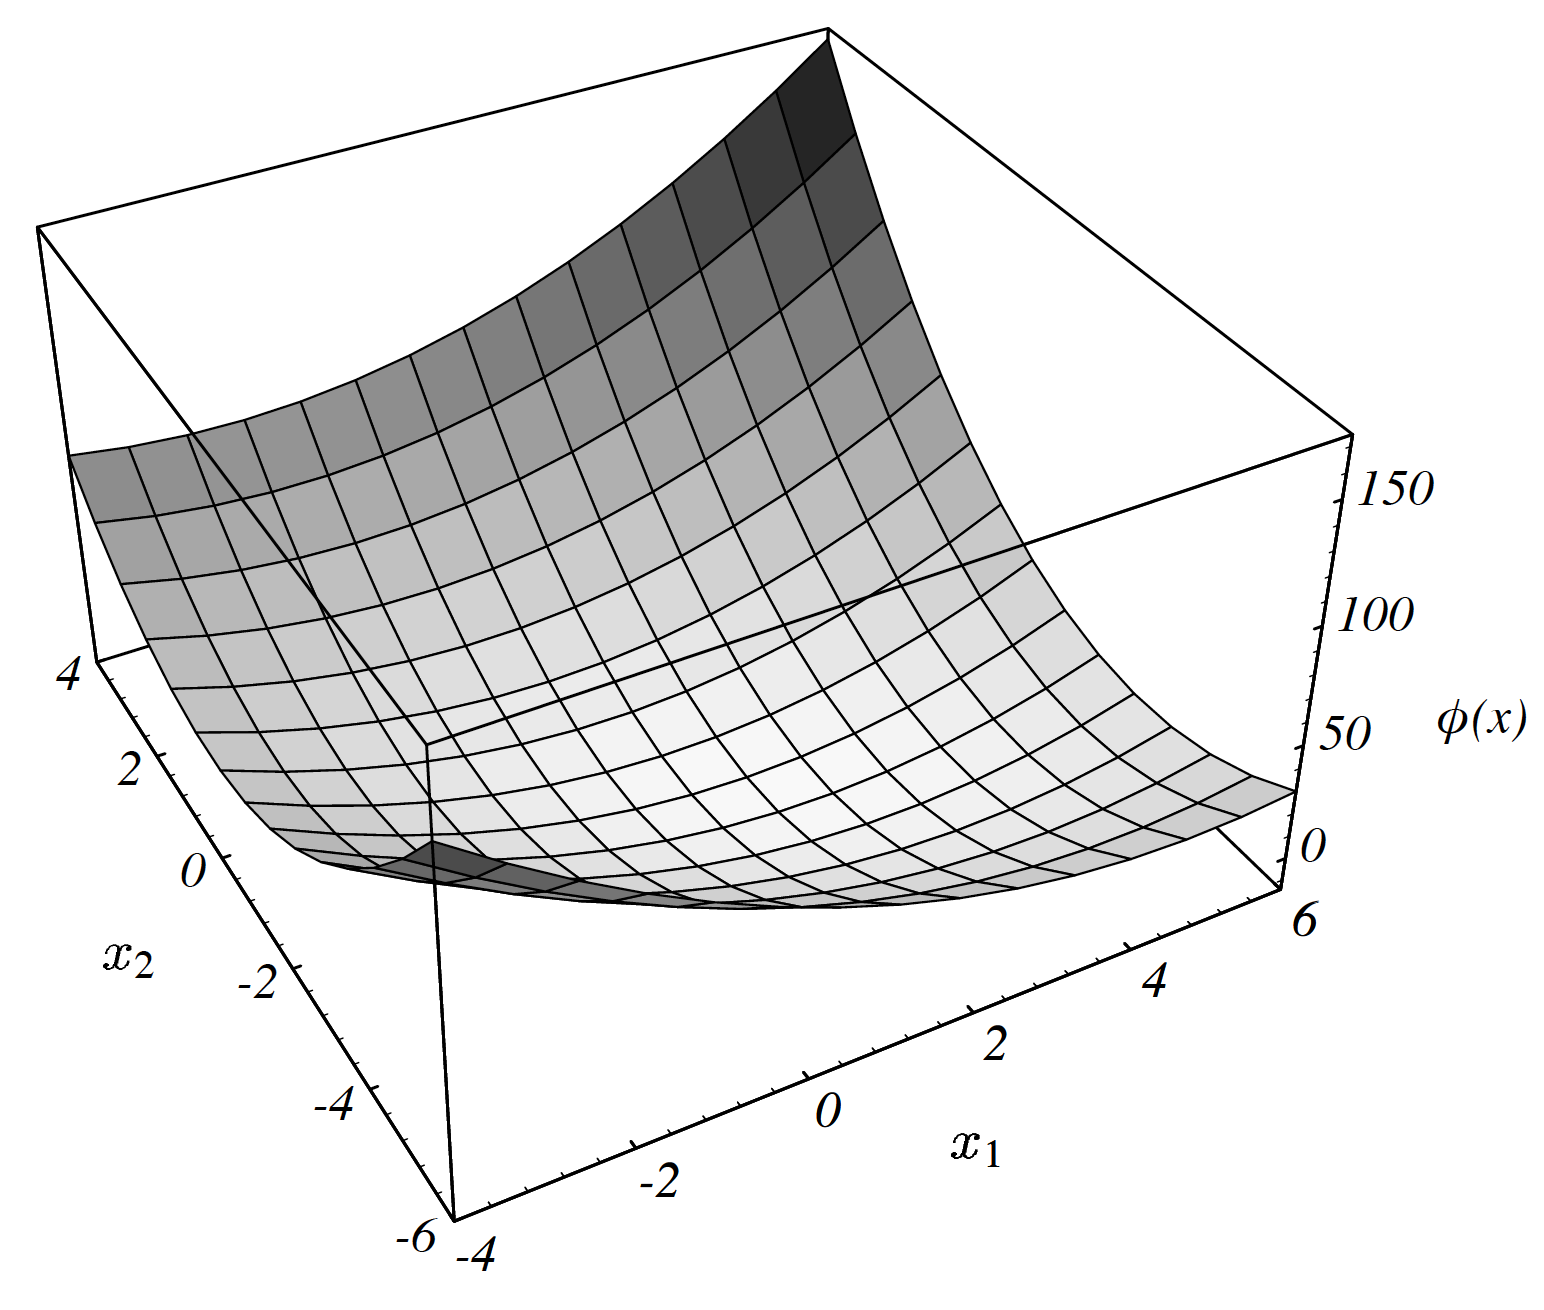
\includegraphics[width=.25\linewidth]{cg_quad.png}
    \caption{Forma quadratica per una matrice definita positiva.}
    \label{fig:quad}
\end{figure}
\end{frame}



\begin{frame} \frametitle{Metodo di discesa (II)}
 \begin{itemize}
 \item Calcolo del gradiente di $\phi(\mathbf{x})$: $\nabla\phi(\mathbf{x}) = A\mathbf{x}-\mathbf{b}$.
 
 \item $\nabla \phi(\mathbf{x}^{\ast})=A\mathbf{x}^{\ast}-\mathbf{b}=\mathbf{0}$: risolvere il problema di minimo su $\phi(\mathbf{x})$ \alert{equivale} quindi a risolvere il sistema A$\mathbf{x}=\mathbf{b}$.

 \item Assegnato un $\mathbf{x}_0\in \mathbb{R}^n$, si procede per ogni $\mathit{k}$ fino a convergenza:
    \begin{enumerate}
        \item determinando una direzione di discesa $\mathbf{d_k} \in \mathbb{R}^n$
        \item determinando un passo $\alpha_k\in \mathbb{R}$
        \item ponendo $\mathbf{x}_{k+1}=\mathbf{x}_{k}+\alpha_k\mathbf{d}_{k}.$
    \end{enumerate}
    
 %\item Condizioni per direzione di discesa: %per una funzione $\phi$ è un vettore d tale che: (in un punto x generico) 
  %   \begin{enumerate}
   %     \item $\mathbf{d}^T\nabla\phi(\mathbf{x}) < 0$, se $\nabla\phi(\mathbf{x})  != 0$
    %    \item $\mathbf{d} = \mathbf{0}$, se $\nabla\phi(\mathbf{x}) = 0$
%    \end{enumerate}

    \item Direzioni di discesa $\mathbf{d}_k$ diverse rispetto al metodo del Gradiente.
    %\begin{itemize}
    %    \item Gradiente $\rightarrow$ $\mathbf{d}_k=-\nabla \phi(\mathbf{x}_k)$
    %    \item Gradiente Coniugato $\rightarrow$ %$\mathbf{d}_k:\mathbf{d}_kA^T\mathbf{d}_{k-1}$
        
    %\end{itemize}

\end{itemize}
\end{frame}


\begin{frame}{Confronto Gradiente Coniugato - Gradiente}
    \begin{figure}
    \centering
    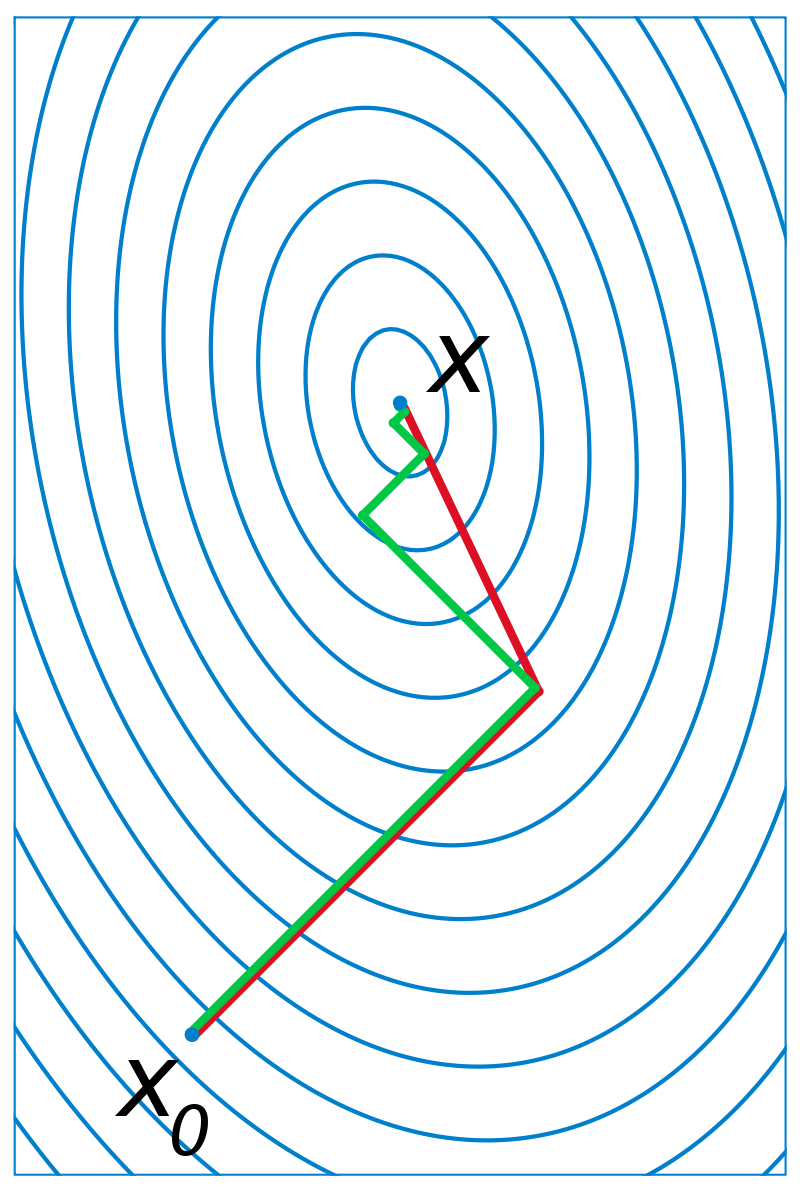
\includegraphics[width=.35\linewidth]{cg_comp.png}
    \caption{Confronto tra il numero di iterazioni dei due metodi ({\color{green}Gradiente}, {\color{red}Gradiente Coniugato}).}

\end{figure}
\end{frame}


\section{Metodo del Gradiente Coniugato}\label{sec:sec2}
\subsection{Direzione di discesa}
\begin{frame} \frametitle{Direzione di discesa}
\begin{itemize}
%\item Affinchè $\{\mathbf{d}_k\}$ siano $A$-ortogonali e ottenute a partire da $\{\mathbf{r}_k\}$  $\mathbf{d}_{j}^TA\mathbf{d}_{k+1}=\mathbf{r}_{k+1}^T\mathbf{d}_j=\mathbf{0}$ per $j=0,\dots,k$
\item Utilizziamo l'\alert{ortogonalizzazione di Gram-Schmidt} per ottenere direzioni %$\{\mathbf{d}_k\}$ 
$A$-ortogonali $\{\mathbf{d}_kA^T\mathbf{d}_{k-1}\}$ a partire dai residui 
%$\{\mathbf{r}_k=\mathbf{b}-A\mathbf{x}_k\}$
\begin{itemize}
\item $\mathbf{d}_0=\mathbf{r}_0$
\item $\mathbf{d}_{k+1}=\mathbf{r}_{k+1}+\sum_{h=0}^k\beta_{kh}\mathbf{d}_h$
\end{itemize}
%\item Dato che $A\mathcal{K}_k$ è incluso in $\mathcal{K}_{k+1}$, il fatto che $\mathbf{r}_{k+1}$ sia ortogonale a $\mathcal{K}_{k+1}$ implica che $\mathbf{r}_{k+1}$ sia $A$-ortogonale a $\mathcal{K}_k$, e quindi a tutte le precedenti direzioni di discesa $\mathbf{d}$, esclusa $\mathbf{d}_k$. 
\item $\mathbf{r}_{k+1} \perp \mathcal{K}_{k+1} \subseteq A\mathcal{K}_k$ implica $\mathbf{r}_{k+1} A$-ortogonale a $\mathcal{K}_k$, e quindi a tutte le precedenti direzioni di discesa $\mathbf{d}$, esclusa $\mathbf{d}_k$. 
\item Le direzioni sono \alert{linearmente indipendenti}
\item \alert{Non è necessario memorizzare le vecchie direzioni} per assicurare la $A$-ortogonalità delle nuove.
\item La \alert{direzione di discesa} diviene
$$
\mathbf{d}_{k+1}=\mathbf{r}_{k+1}+\beta_{k+1}\mathbf{d}_k
\text{ con }\beta_{k+1}=\frac{\mathbf{r}_{k+1}^T\mathbf{r}_{k+1}}{\mathbf{r}_{k}^T\mathbf{r}_{k}}
$$
\item Errori di approssimazione $\rightarrow$ Start\&Stop
\end{itemize}
\end{frame}


%\begin{frame} \frametitle{Scelta della direzione di discesa}
%\begin{itemize}
    
%    \item Scegliamo ad ogni passo una direzione $A$-ortogonale rispetto a tutte le direzioni precedenti, cioè tale che $(A\mathbf{d}_{j})^T\mathbf{d}_{k+1}=\mathbf{0}$ e $(\mathbf{r}_{k+1})^T\mathbf{d}_j=\mathbf{0}$ con $j=0,\dots,k$.
    
 %   \item All'inizio $\mathbf{d}_0=\mathbf{r}_0$, poi $(\mathbf{d}_{k+1})=\mathbf{r}_{k+1}-\beta_k\mathbf{d}_k$ per $k=0,\dots,n-1$, con $\beta_k=\frac{(A\mathbf{d}_{k})^T\mathbf{r}_{k+1}}{(A\mathbf{d}_{k})^T\mathbf{d}_{k}}$ (scelta ottimale).
    
 %   \item In questo modo le $\mathbf{d}_k$ sono linearmente indipendenti e la soluzione $\mathbf{x}_{k+1}$ è ottimale rispetto a tutte le direzioni di discesa (ovvero $\mathbf{r}_{k+1}$ è ortogonale a $\mathbf{d}_k$): è garantito che $\mathbf{x}_n=\mathbf{x}^{\ast}$.
%\end{itemize}
%\end{frame}
\subsection{Passo di discesa}
\begin{frame} 
\frametitle{Passo di discesa}
\begin{itemize}

\item Il passo di discesa più conveniente è quello che \alert{ minimizza $\phi(\mathbf{x_{k+1}})$}

   \item Sostituiamo $\mathbf{x}_{k+1}=\mathbf{x}_{k}+\alpha_k\mathbf{d}_{k}$ nella forma quadratica: \vspace*{13px}
   
   \resizebox{0.9\hsize}{!}{
   $$\phi(\mathbf{x_{k+1}})=\phi(\mathbf{\mathbf{x}_{k}+\alpha_k\mathbf{d}_{k}})=\frac{1}{2}\left(\mathbf{d}_k^TA\mathbf{d}_k\right)\alpha_k^2-\mathbf{d}_k^T\underbrace{\left(\mathbf{b}-A\mathbf{x}_k\right)}_{=\mathbf{r}_k}\alpha_k+\frac{1}{2}\mathbf{x}_k^TA\mathbf{x}_k-\mathbf{x}_k^T\mathbf{b}$$}
   \vspace*{12px}
    
    \item Deriviamo e imponiamo la condizione di stazionarietà:
    $$
    \frac{d\phi}{d\alpha_k}(\mathbf{\mathbf{x}_{k}+\alpha_k\mathbf{d}_{k}})=\left(\mathbf{d}_k^TA\mathbf{d}_k\right)\alpha_k-\mathbf{d}_k^T\mathbf{r}_k=0 $$
    \item Ricaviamo $\alpha_k$:
$$\alpha_k=\frac{\mathbf{d}_k^T \mathbf{r}_k}{\mathbf{d}_k^T A \mathbf{d}_k}$$ .

\end{itemize}
\end{frame}

\begin{frame} \frametitle{Passo di discesa (II)}
\begin{figure}
    \centering
    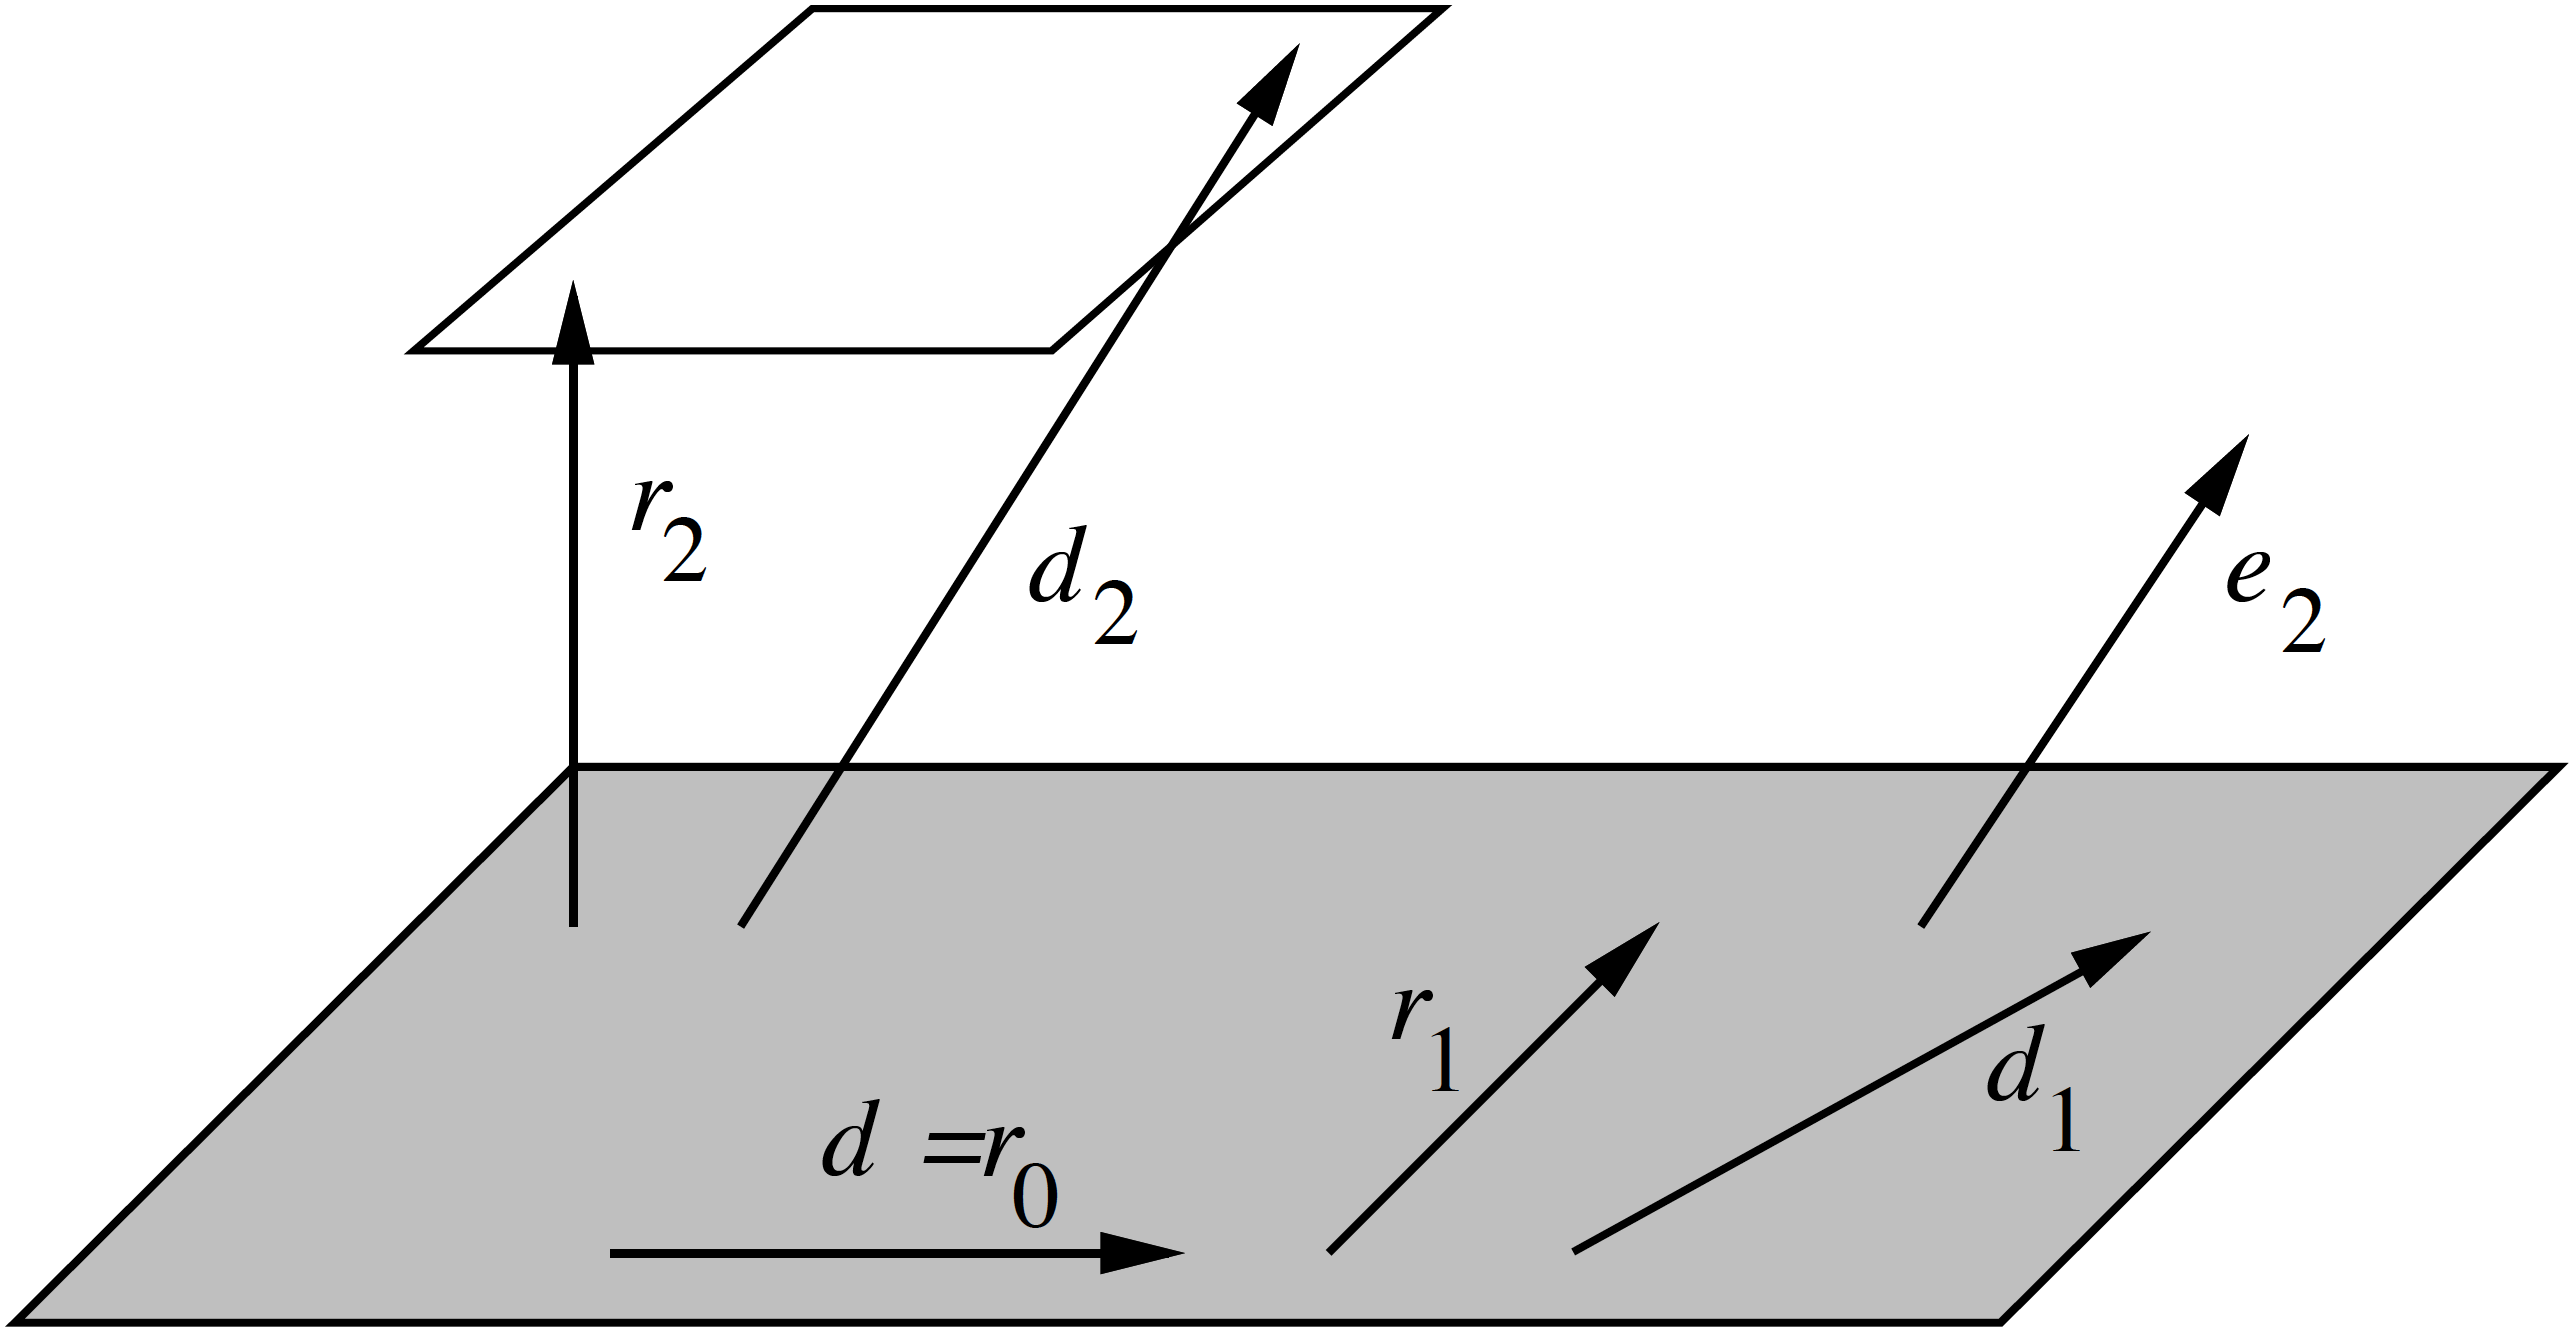
\includegraphics[width=.75\linewidth]{cg_ort.png}
    \caption{Il piano scuro è il sottospazio $\mathcal{K}_2$. Notiamo che $\mathbf{r_2}$ e $\mathbf{d}_2$ puntano su un piano parallelo a $\mathcal{K}_2$ (come conseguenza dell'ortogonalizzazione)}
    \label{fig:ortogonalizzazione}
\end{figure}
\begin{itemize}
\item Se $\mathbf{d}_0=\mathbf{r}_0$ $\Rightarrow$  $\mathbf{d}_k^T\mathbf{r}_k=\mathbf{r}_k^T\mathbf{r}_k$ e otteniamo il \alert{passo di discesa} come
$$
\alpha_k=\frac{\mathbf{r}_k^T \mathbf{r}_k}{\mathbf{d}_k^T A \mathbf{d}_k}
$$
\end{itemize}
\end{frame}



%\begin{frame}\frametitle{Metodo del Gradiente Coniugato come Metodo di Krylov}
%\begin{itemize}
    %\item Il metodo del Gradiente Coniugato può essere visto come un particolare metodo di Krylov: la soluzione $\mathbf{x}^{\ast}$ appartiene al sottospazio di Krylov $\mathcal{K}_\mathrm{n}(A,\mathbf{r}_{(0)})$, e ad ogni iterazione anumenta di dimensione. 
    %\item Le condizioni di ortogonalita del vettore residuo rispetto alle n direzioni di discesa sono espresse nel sottospazio  $\mathcal{L}_\mathrm{n}\subseteq \mathbb{R}^n$, generato da queste ultime (che sono poste indipendenti tra loro): $$\mathcal{L}_\mathrm{n}=span\{ \mathbf{d}_{(0)},\dots,\mathbf{d}_{(n-1)} \} $$.
    
    %\item Si può dimostrare che tale metodo è caratterizzato da iterazione di sottospazi di Krylov
    %\item In particolare usa l’approccio (o classe) di Ritz-Galerkin:
    %\item Costruisce il vettore $\mathbf{x}_k$ tale che il residuo corrispondente sia ortogonale al sottospazio di Krylov con indice 'k', ossia:
    %$\mathbf{r}_k = \mathbf{b} - A\mathbf{x}_k$ normale a $\mathcal{K}_\mathrm{k}$
    
%\end{itemize}
%\end{frame}
\subsection{Velocità di convergenza}
\begin{frame}
\frametitle{Velocità di convergenza}
\begin{itemize}
    \item Il metodo del gradiente coniugato converge al massimo in $\mathrm{n}$ iterazioni (in aritmetica esatta), e si ottiene che %$$\|\mathbf{e}_{(k)}\|_A\leq\frac{2c^k}{1+c^{2k}}\|\mathbf{e}_{(0)}\|_A$$
    $$\|\mathbf{e}_{(k)}\|_A\leq2c^k\|\mathbf{e}_{(0)}\|_A$$
    $$ c=\frac{\sqrt{\kappa_2(A)}-1}{\sqrt{\kappa_2(A)}+1}.$$
    $$\kappa_2(A)\text{ è il numero di condizionamento in norma 2 di } A$$
    \item Come metodo iterativo, viene arrestato quando il residuo relativo $E_{(k)}=\frac{\|\mathbf{r}_{(k)}\|}{\|\mathbf{r}_{(0)}\|}$ è minore di una tolleranza data. 
\end{itemize}
\end{frame}


\begin{frame} \frametitle{Residuo}
\begin{itemize}
\item Calcoliamo il \alert{residuo} $\mathbf{r}_k =\mathbf{b}-A\mathbf{x}_k$: 
$$\mathbf{r}_{k+1}=\mathbf{r}_k-\alpha_kA\mathbf{d}_{k}$$ .

\item Dimostrazione:
\begin{itemize}
    \item $\mathbf{r}_{k+1}=-A\mathbf{e}_{k+1}$
    \item $\mathbf{r}_{k+1}=-A\left(\mathbf{e}_k+\alpha_k\mathbf{d}_k \right)$
    %\item $\mathbf{e}_k=-A^{-1}\mathbf{r}_k \right)$
    \item $\mathbf{r}_{k+1}=\mathbf{r}_k-\alpha_kA\mathbf{d}_{k}$
    
    \end{itemize}

\item Errori di approssimazione $\rightarrow$ utilizzare $\mathbf{r}_k =\mathbf{b}-A\mathbf{x}_k$ ogni tot iterazioni
\end{itemize}
\end{frame}
\subsection{Implementazione}
\begin{frame}
\frametitle{Metodo del gradiente coniugato}
\begin{itemize}
\item $k=0$
\begin{itemize}
\item $\mathbf{d}_0=\mathbf{r}_0=\mathbf{b}-A\mathbf{x}_0$
\end{itemize}   
\item $k>0$
\begin{itemize}
\item $\alpha_k=\frac{\mathbf{r}_k^T \mathbf{r}_k}{\mathbf{d}_k^T A \mathbf{d}_k}$
\item $\mathbf{x}_{k+1}=\mathbf{x}_k+\alpha_k\mathbf{d}_{k}$
\item $\mathbf{r}_{k+1}=\mathbf{r}_k-\alpha_kA\mathbf{d}_{k}$
\item $\beta_{k+1}=\frac{\mathbf{r}_{k+1}^T\mathbf{r}_{k+1}}{\mathbf{r}_{k}^T\mathbf{r}_{k}}$
\item $\mathbf{d}_{k+1}=\mathbf{r}_{k+1}+\beta_{k+1}\mathbf{d}_k$
\end{itemize}  
\end{itemize}    
\end{frame}

\begin{frame}\frametitle{Implementazione Matlab}

Dati come input
una matrice \lstinline[language=Matlab]{A}, 
il vettore dei termini noti \lstinline[language=Matlab]{b},
una guess iniziale \lstinline[language=Matlab]{x},
un numero massimo di iterazioni \lstinline[language=Matlab]{kmax}
e una tolleranza \lstinline[language=Matlab]{e}
\lstinputlisting[language=Matlab]{gradienteconiugato.m}
\end{frame}
\subsection{Precondizionamento}
\begin{frame}
\frametitle{Precondizionamento (I)}
\begin{itemize}
    %\item La velocità di convergenza dipende quindi dal numero di condizionamento $\mathit{K(A)}$. %più è grande ka piu lenta conv.
    
    \item $M: K(M^{-1}A)\ll K(A)$
    \item \alert{Sistema precondizionato} (equivalente a $A\mathbf{x}=\mathbf{b}$)
    $$
    M^{-1}A\mathbf{x}=M^{-1}\mathbf{b}
    $$
    \item $M$ e $A$ simmetriche e definite $\nRightarrow$ $M^{-1}A$ simmetrica e definita
    \item $\forall M$ simmetrica e definita positiva $\Rightarrow \exists P : PP^T=M$.
    \item $M^{-1}A$ e $P^{-1}AP^{-T}$ hanno gli stessi autovalori, allora:
    $$
    P^{-1}AP^{-T}\mathbf{\hat{x}}=P^{-1}\mathbf{b},\, \mathbf{\hat{x}}=P^T\mathbf{x}
    $$
    
    \item $P^{-1}AP^{-T}$ è simmetrica e definita positiva $\Rightarrow$ CG applicabile
    \item $M^{-1}=P^{-T}P^{-1}$
    
\end{itemize}    
\end{frame}


\begin{frame}
\frametitle{Precondizionamento (II)}
\begin{itemize}
    \item Scegliendo $M$ stiamo operando un \textit{trade-off} tra la diminuzione del numero di condizionamento e il costo computazionale della risoluzione del calcolo del residuo precondizionato $\mathbf{s_{(k)}}=M^{-1}\mathbf{r_{(k)}}$.
    \item Esempio:
    \begin{itemize}
    \item Precondizionamento di Jacobi
    \end{itemize}    
   
    %\item  La convergenza del metodo precondizionato è più veloce, poichè $K(A) \rightarrow K(M^{-1}A)$:
    %$$\|\mathbf{e}_{(k)}\|_A\leq\frac{2c^k}{1+c^{2k}}\|\mathbf{e}_{(0)}\|_A,  c=\frac{\sqrt{K(P^{-1}A)}-1}{\sqrt{K(P^{-1}A)}+1}.$$
\end{itemize}    
\end{frame}


%\begin{frame}
%frametitle{Metodo del gradiente coniugato (con precondizionamento)}
%\begin{itemize}
%\item $\mathbf{r}_0=\mathbf{b}-A\mathbf{x}_0$
%\item $\mathbf{d}_0=M^{-1}\mathbf{r}_0$
%\item $\alpha_k=\frac{\mathbf{r}_k^TM^{-1} \mathbf{r}_k}{\mathbf{d}_k^T A \mathbf{d}_k}$
%\item $\mathbf{x}_{k+1}=\mathbf{x}_k+\alpha_k\mathbf{d}_{k}$
%\item $\mathbf{r}_{k+1}=\mathbf{r}_k-\alpha_kA\mathbf{d}_{k}$
%\item $\beta_{k+1}=\frac{\mathbf{r}_{k+1}^TM^{-1}\mathbf{r}_{k+1}}{\mathbf{r}_{k}^TM^{-1}\mathbf{r}_{k}}$
%\item $\mathbf{d}_{k+1}=M^{-1}\mathbf{r}_{k+1}+\beta_{k+1}\mathbf{d}_k$
%\end{itemize}    
%\end{frame}

%\begin{frame}\frametitle{Implementazione Matlab (con precondizionamento)}
%Dati come input una matrice \lstinline[language=Matlab]{A},  il vettore dei termini noti \lstinline[language=Matlab]{b}, una guess iniziale \lstinline[language=Matlab]{x}, la matrice di precondizionamento \lstinline[language=Matlab]{M}, un numero massimo di iterazioni \lstinline[language=Matlab]{kmax} e una tolleranza \lstinline[language=Matlab]{e} \lstinputlisting[language=Matlab]{gradienteconiugatoprecondizionato.m}
%\end{frame}




\section{GMRES}\label{sec:sec3}


\begin{frame} 
\begin{center}
\begin{tabular}{ c }
\hline\\
\textbf{Generalized Minimal RESidual} \\ [0.5ex]
risoluzione di un sistema lineare tramite sottospazio di Krylov\\ \\
 \hline
\end{tabular}
\end{center}
\end{frame}

\begin{frame} \frametitle{GMRES} 
\begin{itemize}
    \item $A\mathbf{x} = \mathbf{b}$
\item $\mathbf{x}_\mathrm{k}$ è la \alert{soluzione approssimata} del sistema
\item Problema: \alert{minimizzare}      $$\|\mathbf{r}_\mathrm{k}\| = \|\mathbf{b} - A\mathbf{x}_\mathrm{k}\|$$
    \item Osserviamo che $\mathbf{x}_\mathrm{k} \in   \mathcal{K}_\mathrm{k}$ quindi$$\mathbf{x}_\mathrm{k} = \mathcal{K}_\mathrm{k}\mathbf{c}$$ (con $\mathbf{c} \in \mathbb{R}^\mathrm{k}$)
    \item Sostituiamo nella norma $$\|\mathbf{r}_\mathrm{k}\| = \|A\mathcal{K}_\mathrm{k}\mathbf{c} - \mathbf{b}\|$$(risolvibile con fattorizzazione QR di $A\mathcal{K}_\mathrm{k}$).
\item \alert{Difetto}: errori di troncamento in fattorizzazione QR e si genera la matrice $\mathcal{R}$ inutilmente.
\end{itemize}
\end{frame}

%\begin{frame}{GMRES come MK}
 % \begin{itemize}
   %   \item il GMRES è metodo di Krylov, quindi usa uno dei 4 approcci che li caratterizzano
%      \item In particolare usa l’approccio (o classe) del residuo di norma minima: identificare l’$\mathbf{x}_k$ per cui la norma Euclidea (norma 2) del residuo sia minima su  $\mathcal{K}_\mathrm{k}$

%  \end{itemize}  
%\end{frame}
\subsection{Iterazione di Arnoldi}
\begin{frame} \frametitle{L'iterazione di Arnoldi (I)}
\begin{itemize}
    
\item  Definiamo $\mathcal{Q}_\mathrm{k}$ la matrice i cui vettori formano una \alert{base ortonormale} di $\mathcal{K}_\mathrm{k}$; quindi $$\mathcal{K}_\mathrm{k}\mathbf{c} = \mathcal{Q}_\mathrm{k}\mathbf{y}$$
\item   Il problema consiste ora nella ricerca di $\mathbf{y}\in\mathbb{R}^\mathrm{k}$ tale per cui: $$\|A\mathcal{Q}_\mathrm{k}\mathbf{y}-\mathbf{b}\| = minimo$$
\item Definiamo la matrice di Hessenberg $\mathcal{H}_\mathrm{n}$ la matrice quadrata quasi triangolare: $$\begin{bmatrix} h(1,1) & h(1,2) & ... & h(1,n) \\ h(2,1) & h(2,2) & ... & h(2,n) \\0 & h(3,2) & ... & h(3,n) \\ 0 & 0 & ... & ... \\  0& 0&0& h(n,n) \\ \end{bmatrix}$$
\item Consideriamo la sezione superiore sinistra di $\mathcal{H}_\mathrm{n}$ e la chiamiamo $\mathcal{H}_\mathrm{k}$; dim($\mathcal{H}_\mathrm{k}$) = (k+1) x k
 %   \item Con Arnoldi dimostriamo che $A\mathcal{Q}_\mathrm{k} = \mathcal{Q}_{\mathrm{k}+1}\mathcal{H}_\mathrm{k}$ (con $\mathcal{H}_\mathrm{k}$ la matrice alta-sinistra, $(k+1) \ x \ k$, della matrice di Hessenberg). Il problema diventa:$$\|\mathcal{Q}_{\mathrm{k}+1}\mathcal{H}_\mathrm{k}\mathbf{y}-\mathbf{b}\| = minimo.$$ 
\end{itemize}
\end{frame}

\begin{frame}\frametitle{L'iterazione di Arnoldi (II)}

Vediamo un algoritmo matlab per generare  $\mathcal{Q}_\mathrm{k}$ e $\mathcal{H}_\mathrm{k}$ \\ \lstinputlisting[language=Matlab]{Arnoldi.m}

\end{frame}

\begin{frame} \frametitle{L'iterazione di Arnoldi (III)}
\begin{itemize}
\item Riprendendo l'ultima linea di codice $$\mathbf{q}_{\mathrm{k}+1} =\frac{ A \mathbf{q}_{\mathrm{k}}}{\mathbf{h}_{\mathrm{k}}}$$
\item Che diventa $$  A\mathbf{q}_\mathrm{k}  = \mathbf{q}_{\mathrm{k}+1}\mathbf{h}_\mathrm{k} $$
\item Si ricava $$   A\mathcal{Q}_\mathrm{k}  = \mathcal{Q}_{\mathrm{k}+1}\mathcal{H}_\mathrm{k} $$
\item La norma sarà$$\|\mathcal{Q}_{\mathrm{k}+1}\mathcal{H}_\mathrm{k}\mathbf{y}-\mathbf{b}\| = minimo$$
\end{itemize}
\end{frame}


\begin{frame} \frametitle{L'iterazione di Arnoldi (IV)}
\begin{itemize}
    \item Moltiplichiamo entrambi i membri per $\mathcal{Q}^T_{\mathrm{k}+1}$: $$\|\mathcal{H}_\mathrm{k}\mathbf{y}-\mathcal{Q}^T_{\mathrm{k}+1}\mathbf{b}\| = minimo.$$
    \item Osserviamo che $\mathcal{Q}^T_{\mathrm{k}+1}\mathbf{b}=\|\mathbf{b}\|\mathbf{e_1}$, con $\mathbf{e_1}=(1,0,0,\dots)^T$, il problema 
    finale è:$$\|\mathcal{H}_\mathrm{k}\mathbf{y}-\|\mathbf{b}\|\mathbf{e}_1\| = minimo.$$ Risolvibile con l'approssimazione ai minimi quadrati. 
\item Grazie all' \alert{Iterazione di Arnoldi}:\begin{itemize}
\item Inizio da problema di dimensione m x m non ridotto ai minimi quadrati
\item Giungo a problema di dimensione (k+1) x k (o al più (n+1) x n) ridotto ai minimi quadrati \end{itemize}
\end{itemize}
\end{frame}



%\begin{frame} 
%\begin{center}
%\begin{tabular}{ c }
%\hline\\
% \textbf{Analisi stazionaria efficiente} \\ [0.5ex]
%  \textbf{basata sul metodo matrix-free nei sottospazi di Krylov}\\ \\
% \hline
%\end{tabular}
%\end{center}
%\end{frame}


\subsection{Esempio applicativo}
\begin{frame}
\frametitle{Metodi di Krylov nell'elettronica}\framesubtitle{Esempio applicativo su \textbf{circuiti analogici}}
\begin{itemize}
\item Più circuiti $\to$ più problemi per risolverli
\item Risposta del circuito dipende dagli ingressi (ampiezze, frequenze) $\to$ migliaia di punti da verificare
\item $N$ equazioni nel circuito$\to$ $N^3$ flops per Gauss, $N^2$ flops per metodi iterativi$\to N$ flops per GMRES matrix free
\item Matrix-Free VS Iterativi: se $N$=400 $t_{It} \approx 10t_{MF}$
\end{itemize}
\end{frame}

\begin{frame}\frametitle{Metodi di Krylov nell'elettronica}\framesubtitle{\textbf{Matrix Free}}

\begin{figure}
    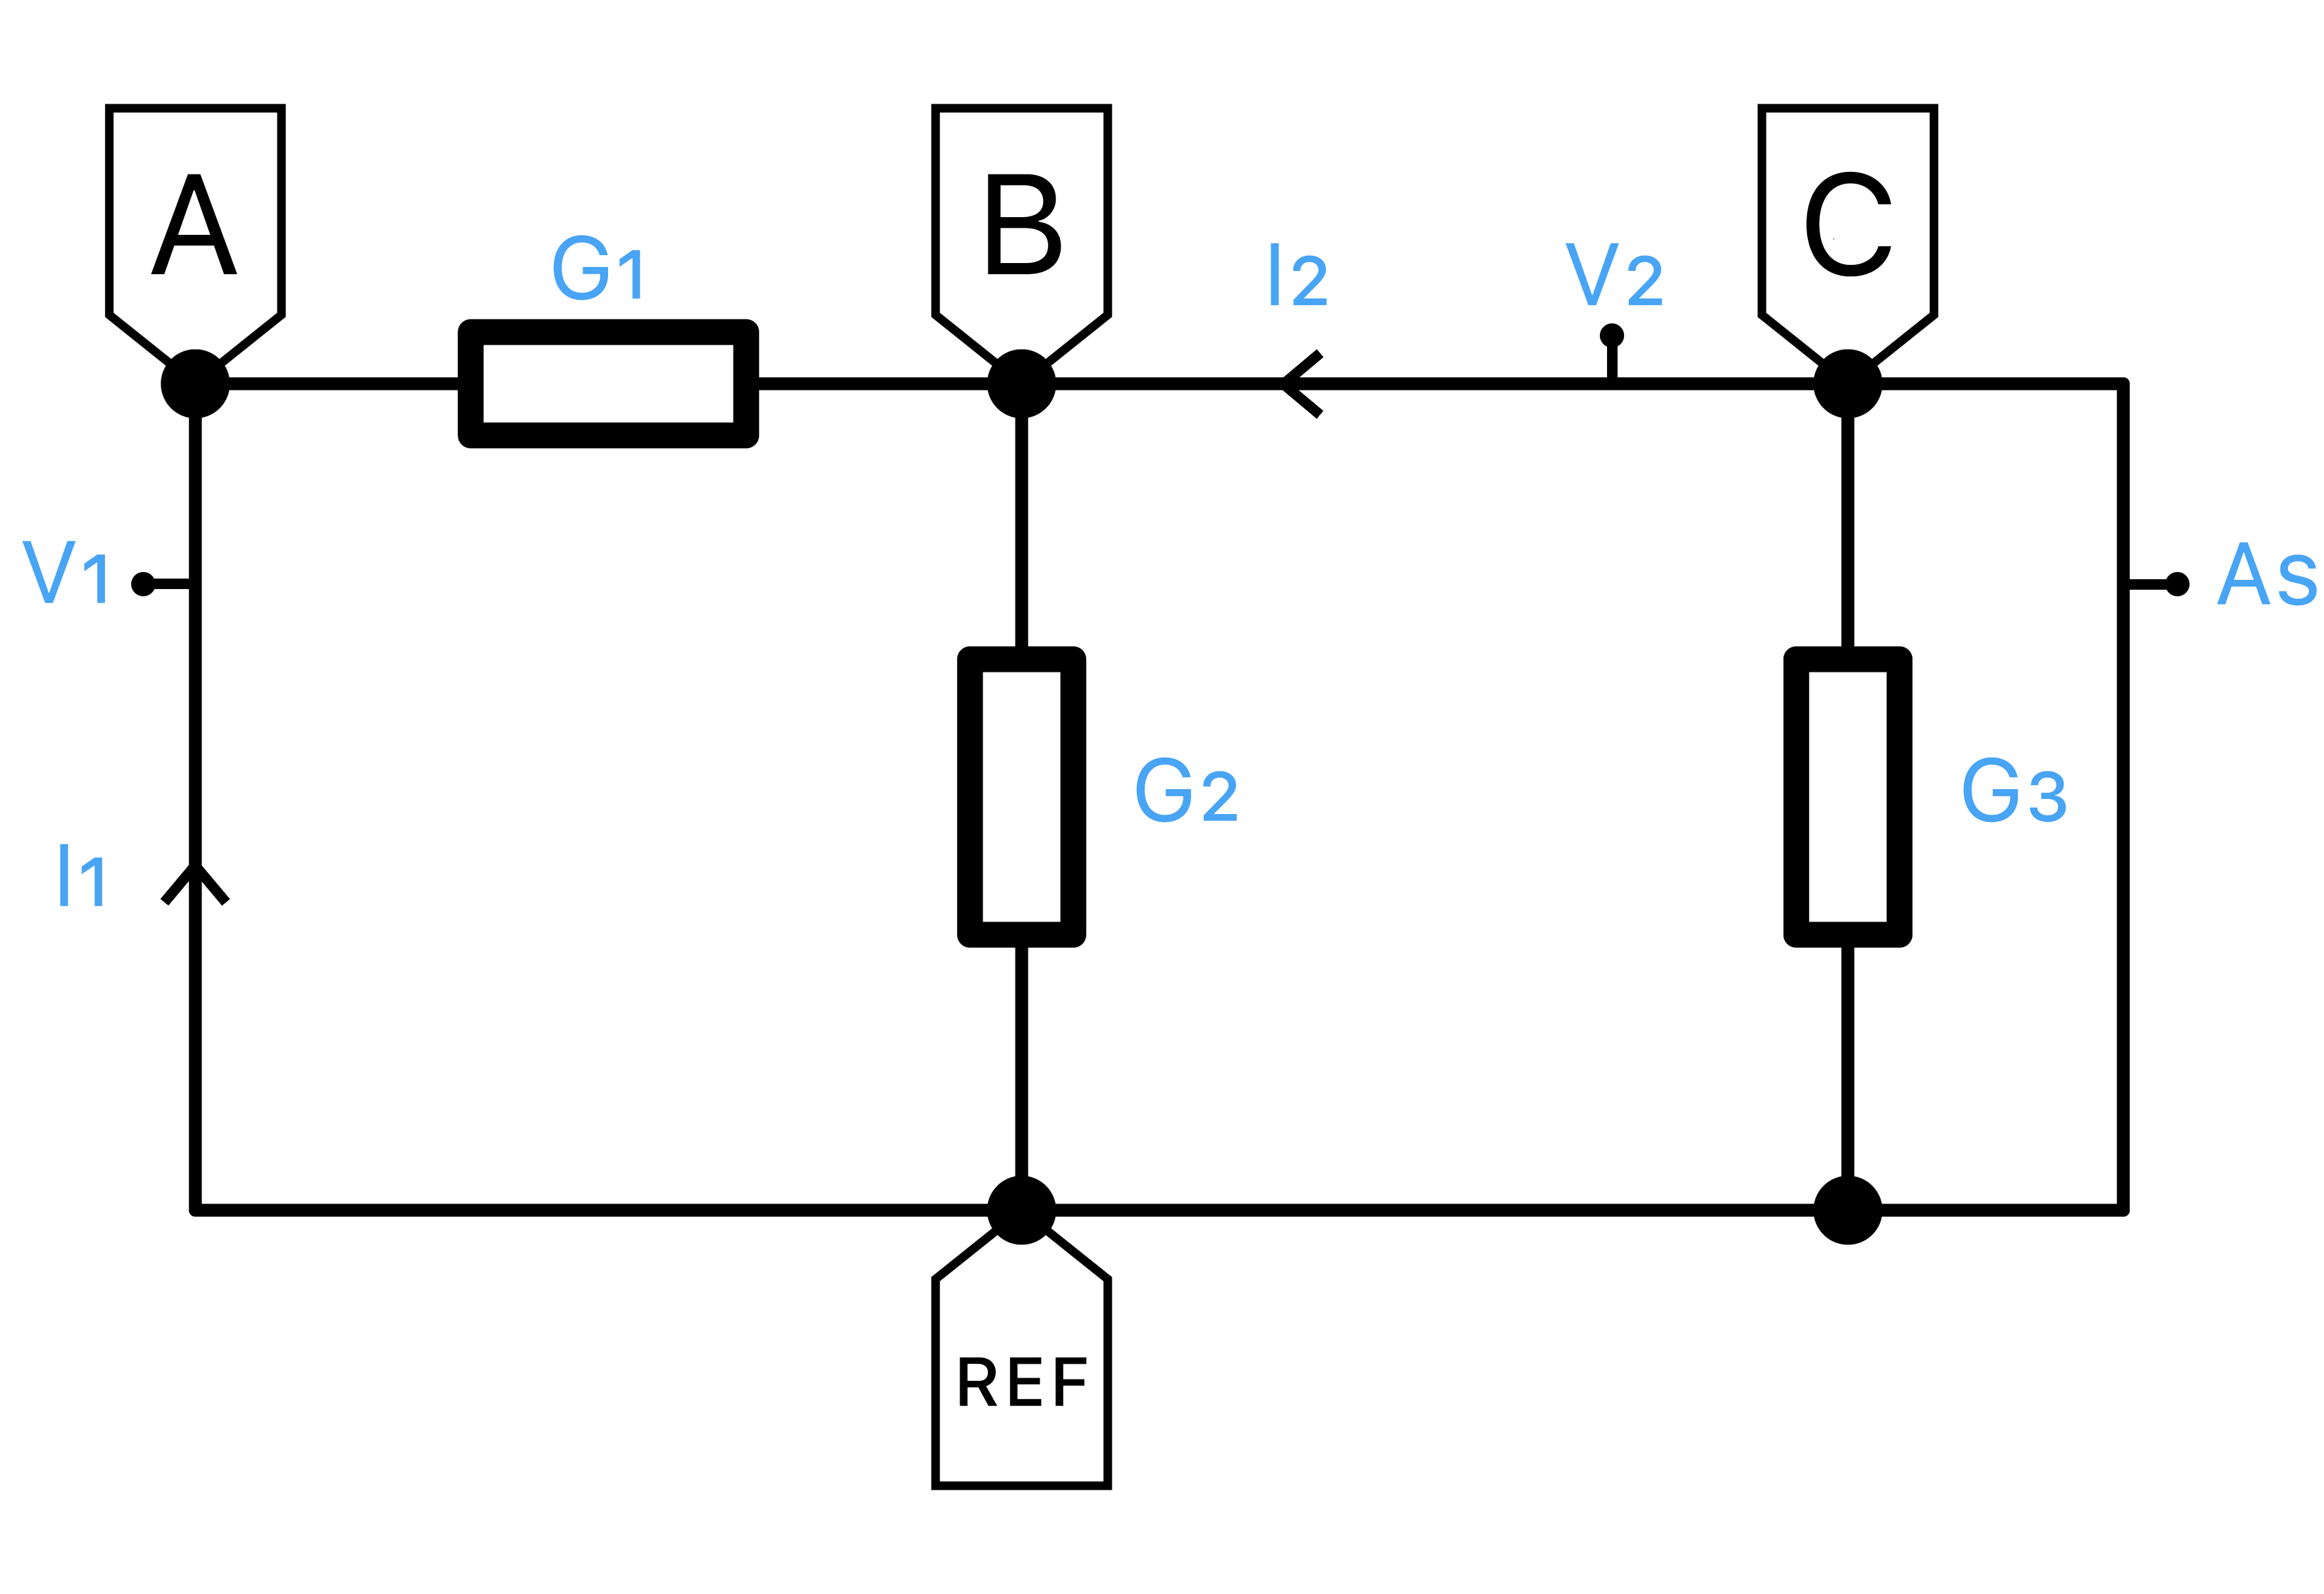
\includegraphics[width=.90\linewidth,height=4.5cm,keepaspectratio]{my_circuit.png}
\end{figure}

$\begin{bmatrix}
G_1 & -G_1 & 0 & -1 & 0 \\ -G_1 & G_1 + G_2 & 0 & 0 & 1 \\ 0 & 0 & G_3 & 0 & -1 \\ -1 & 0 & 0 & -1 & 0 \\ 0 & 1 & -1 & 0 & 0
\end{bmatrix} \ \ \ \begin{bmatrix}V_{A,REF} \\ V_{B,REF} \\ V_{C,REF}\\ i_1 \\ i_2\end{bmatrix} \ \  = \ \ \begin{bmatrix} 0 \\ 0\\ -A_s\\ V_1 \\ V_2 \end{bmatrix}$
\\ \centering $A  \ \ \ \ \ \ \ \ \ \ \ \ \ \ \ \ \ \ \ \ \ \ \ \ \ \ \ \ \ \ \ \ \mathbf{x} \ \ \ \ \ \ \ \ \ = \ \ \  \ \ \ \ \mathbf{b}$
\begin{itemize}

\end{itemize}

\end{frame}

\begin{frame}\frametitle{Metodi di Krylov nell'elettronica}\framesubtitle{\textbf{Matrix Free}}

\begin{figure}
    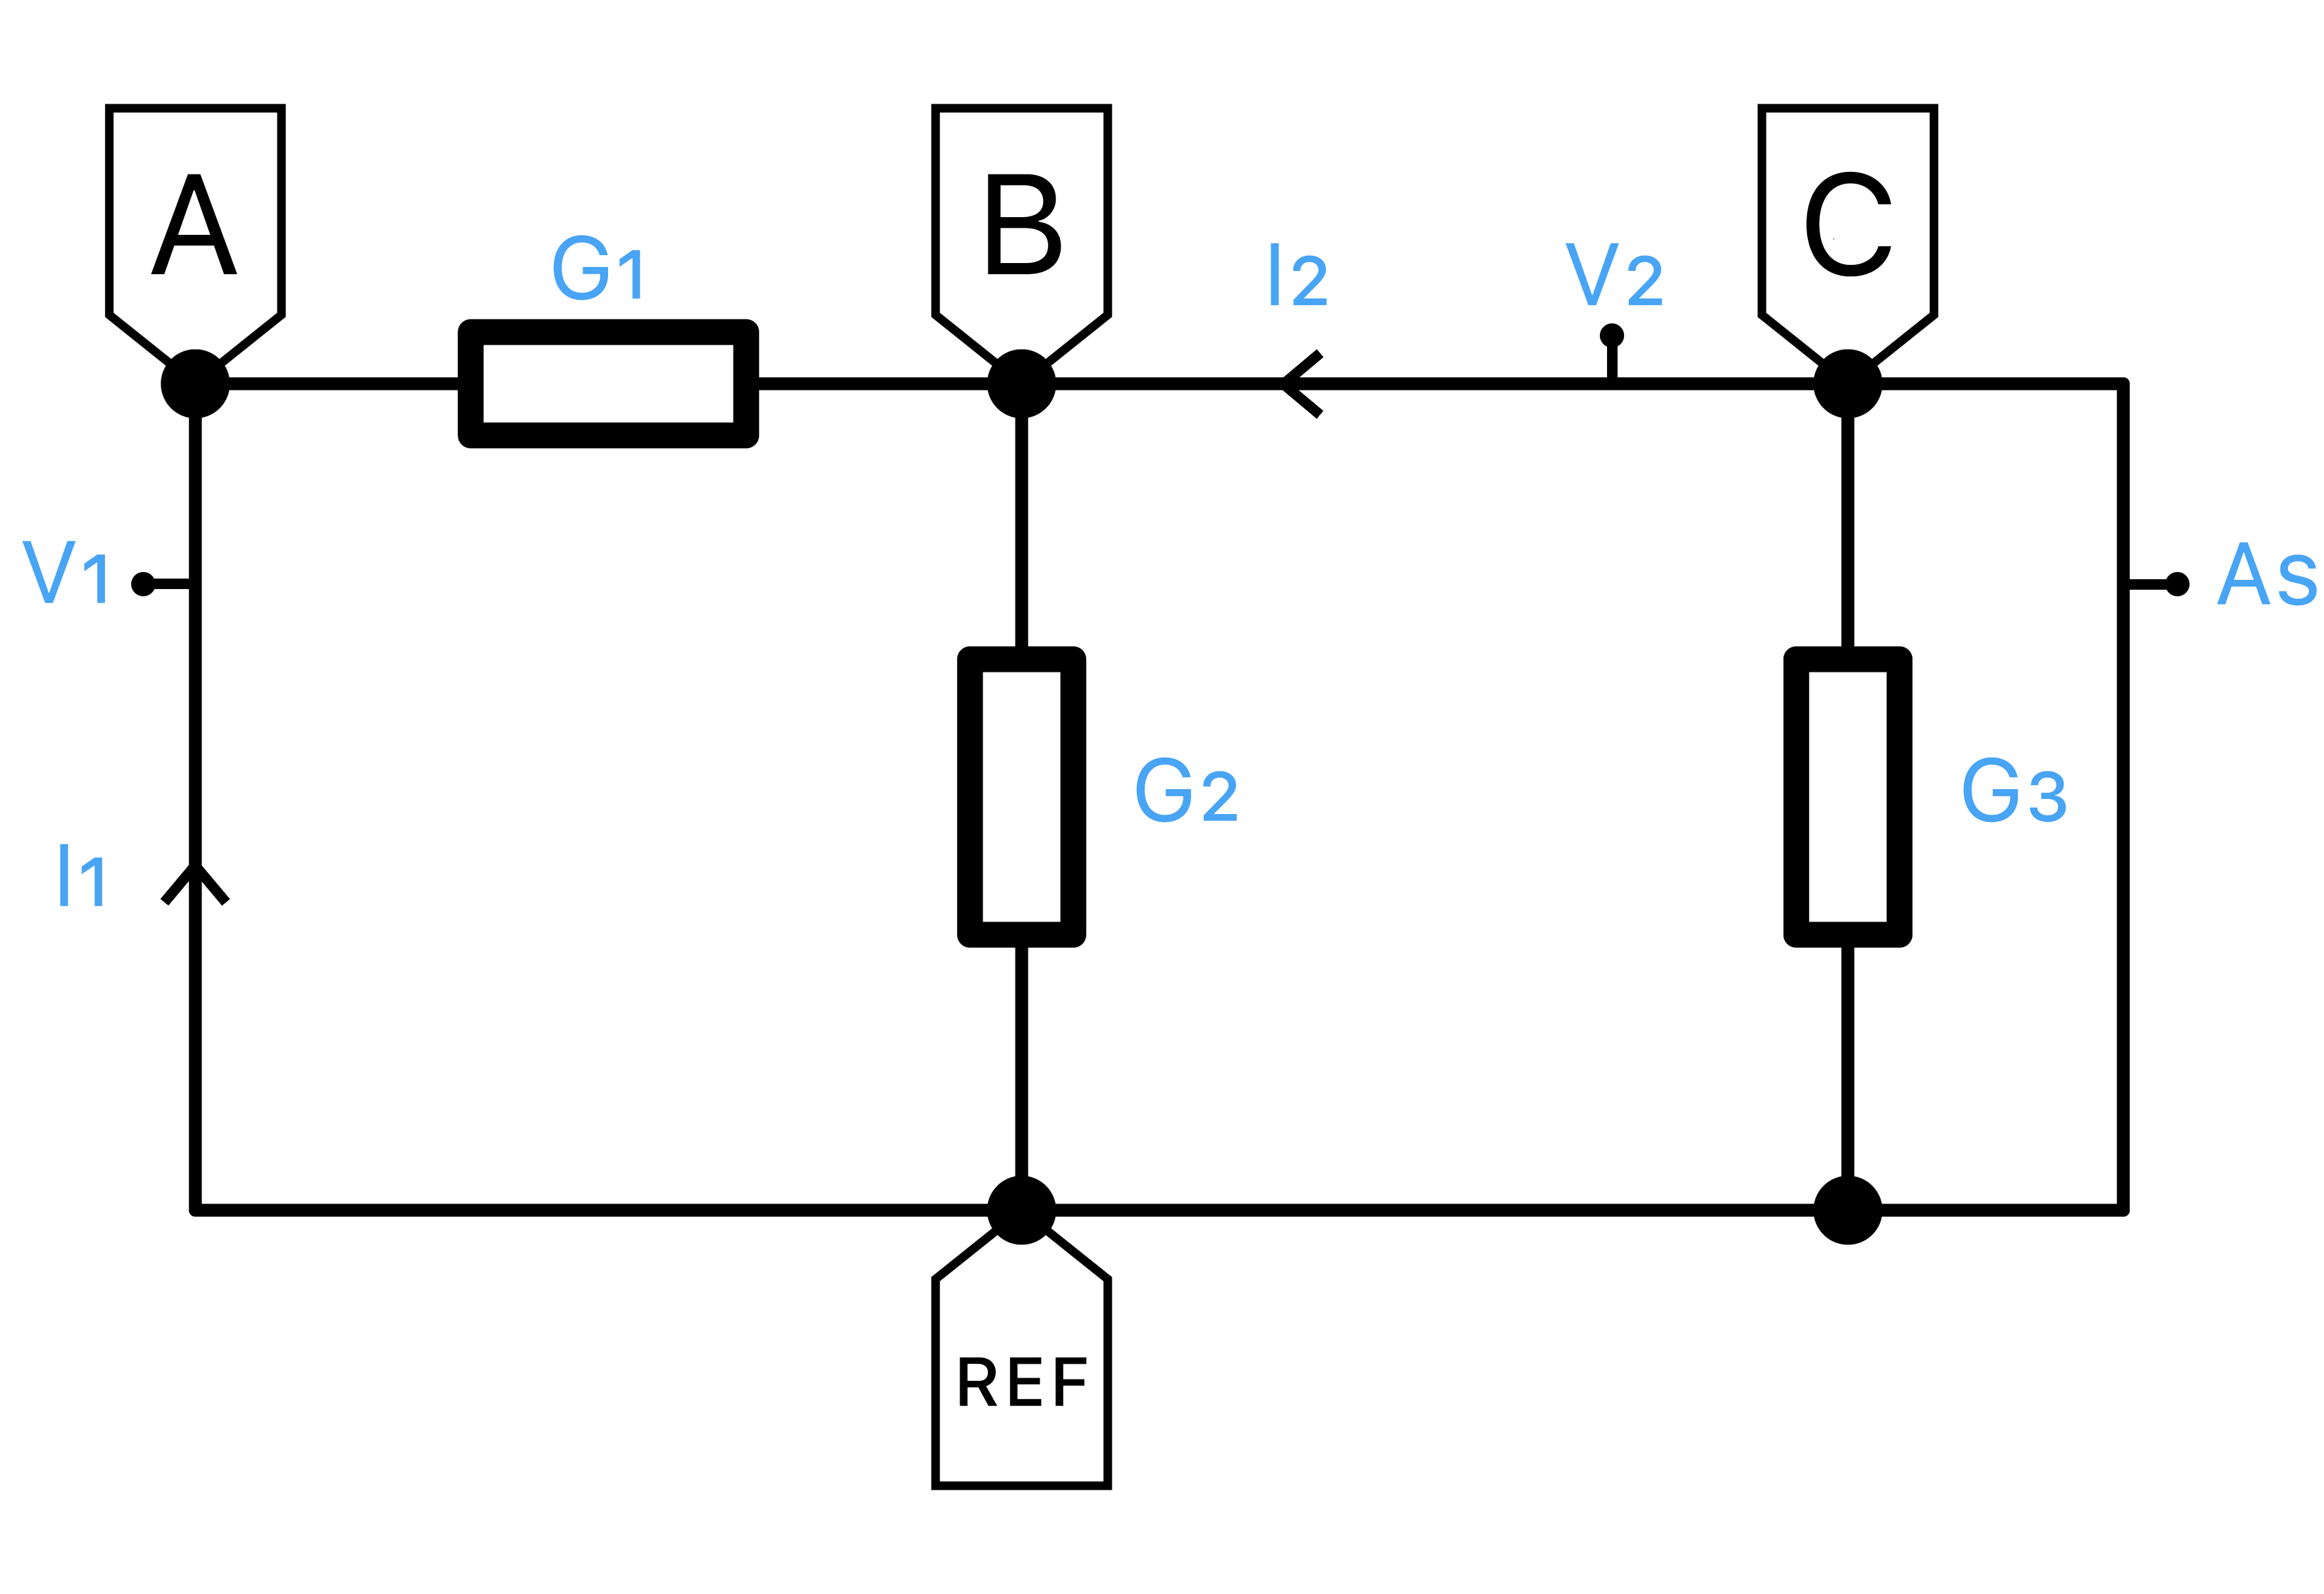
\includegraphics[width=.90\linewidth,height=4.5cm,keepaspectratio]{my_circuit.png}
\end{figure}


\begin{itemize}
\item Circuito piccolo (3 nodi) $\to$ A in forma sparsa
\item Il GMRES Matrix Free non memorizza ogni valore di A $\to$ passo da $N^2$ a $N$ flops
\item Si memorizza: $<a_{i,j}, i, j>$  ($a =$ valore, $i =$ numero di riga, $j =$ numero di colonna)

\end{itemize}
\end{frame}

\begin{frame} \frametitle{Matrix Free GMRES}
\begin{figure}
    \centering
    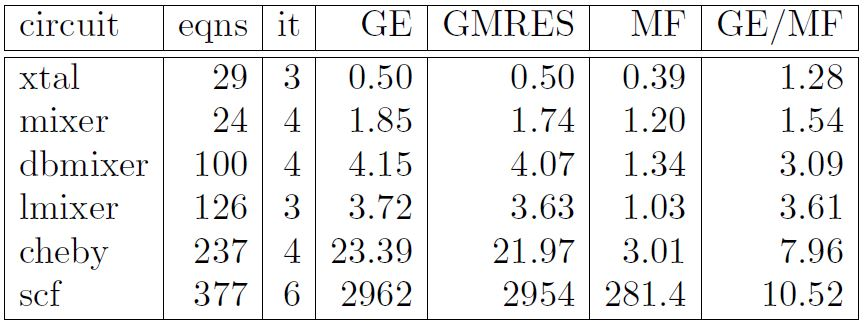
\includegraphics[width=.75\linewidth]{Tabella1.JPG}
    \caption{Comparazione\footnotemark di metodi diversi per la risoluzione dei circuiti elettronici.}
%    \label{fig:my_label}
\end{figure}
%Se la figura ha un'etichetta la si può usare per fare riferimento
%alla figura nel testo : Figura~\ref{fig:my_label}
\footnotetext{Risultati ottenuti con workstation HP 712/80.}
\end{frame}
\end{document}